\subsection{Performance Requirements}
\begin{itemize}
    \item Since the admin side does not handle the execution side of the project. Little to no performance requirements are needed.
    \item All that is needed is a decent connection to the system from the admin to the server at times when nodes are being used. If there is an emergency, then the admin needs to be able to kill nodes.

\end{itemize}
\subsection{Design Constraints}
\begin{enumerate}
	\item The admin needs connection to the system at all times and this can't be ensured.
    \item A connection must be able to be obtained between the system and the database.
    \item There also needs to be a connection maintain between the nodes and the system.

\end{enumerate}
\subsection{Software System Attributes}
Availability:  The admin should be able to access the system at any computer since it is a web app. The admin controls would only be allocated to those that were made admin and also only if they were granted certain privileges such as being able to kill a node or create a user.


\subsection{Class diagram}
 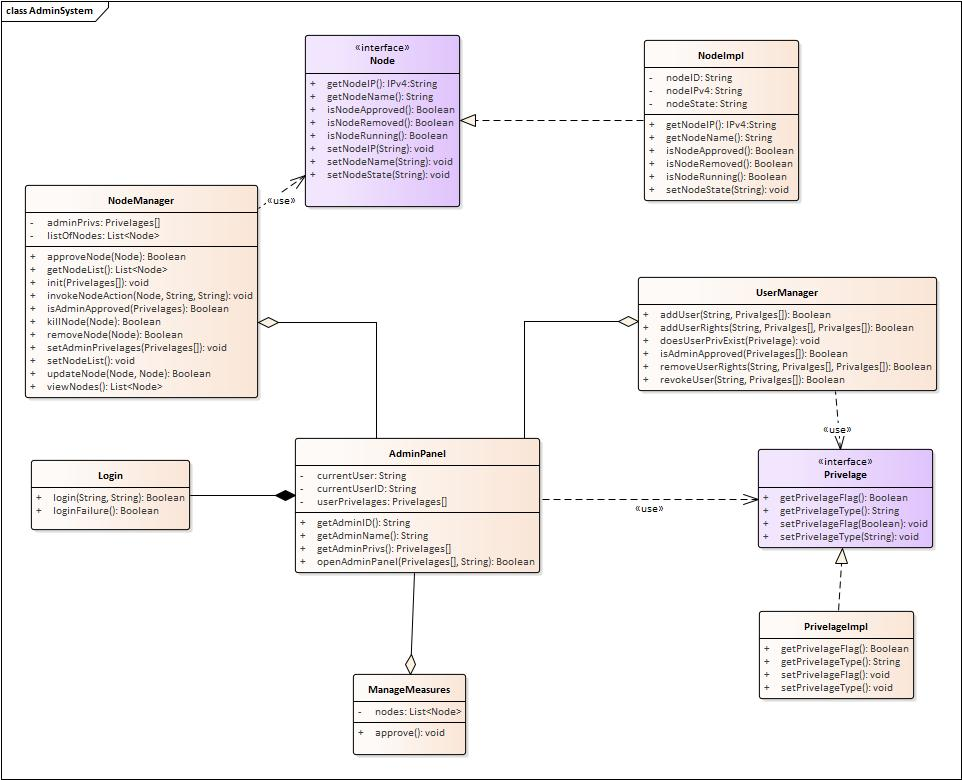
\includegraphics[width=12cm,height=15cm,keepaspectratio]{admin_ui/images/AdminSystem.jpg}
	\begin{center}
	    \small{Figure 25: Class diagram for Admin UI}
    \end{center}
    \par \textbf{Design Patterns Used}
    I used the Façade strategy as the idea was to simplify the Admin interface and interaction to the web component. As most operations will occur on the back end systems the idea is to keep the user blind from what is happening at the back end. Making their lives much less complicated. With a simple press of a button most of all the work is done. \newline \newline
	
	
		
\subsection{Activity diagram}
    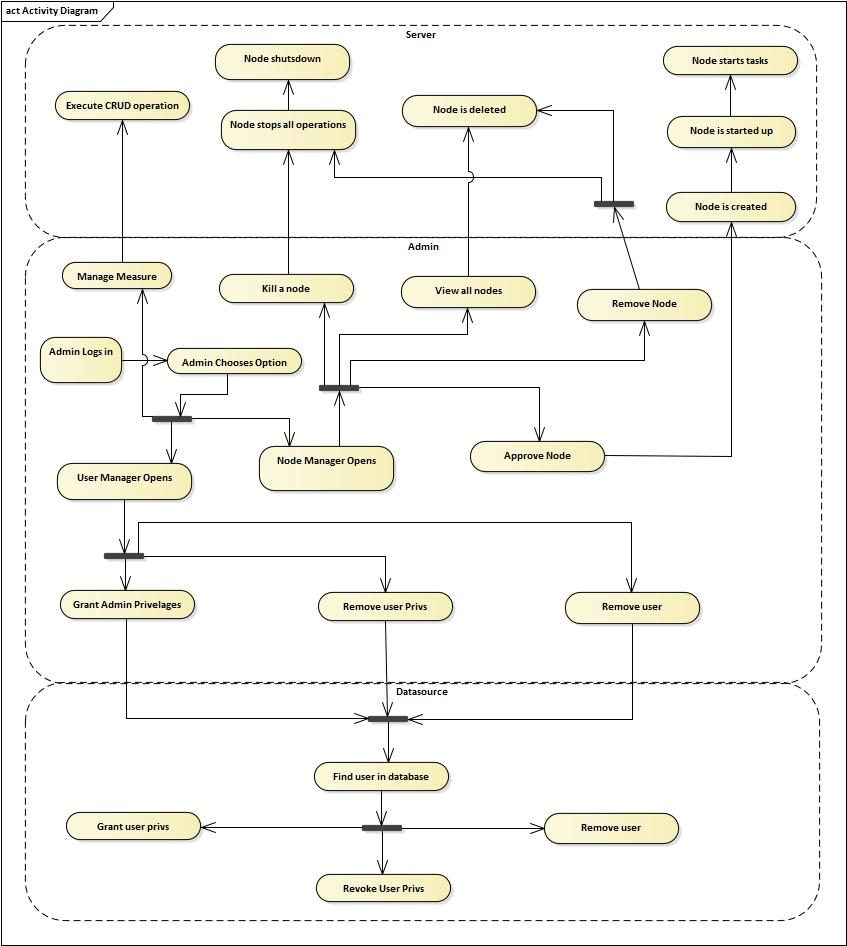
\includegraphics[width=12cm,height=15cm,keepaspectratio]{admin_ui/images/Activity_Diagram.jpg}
	\begin{center}
	    \small{Figure 26: Activity diagram for Admin UI}
    \end{center}


\subsection{Sequence diagrams}
    \bigskip
    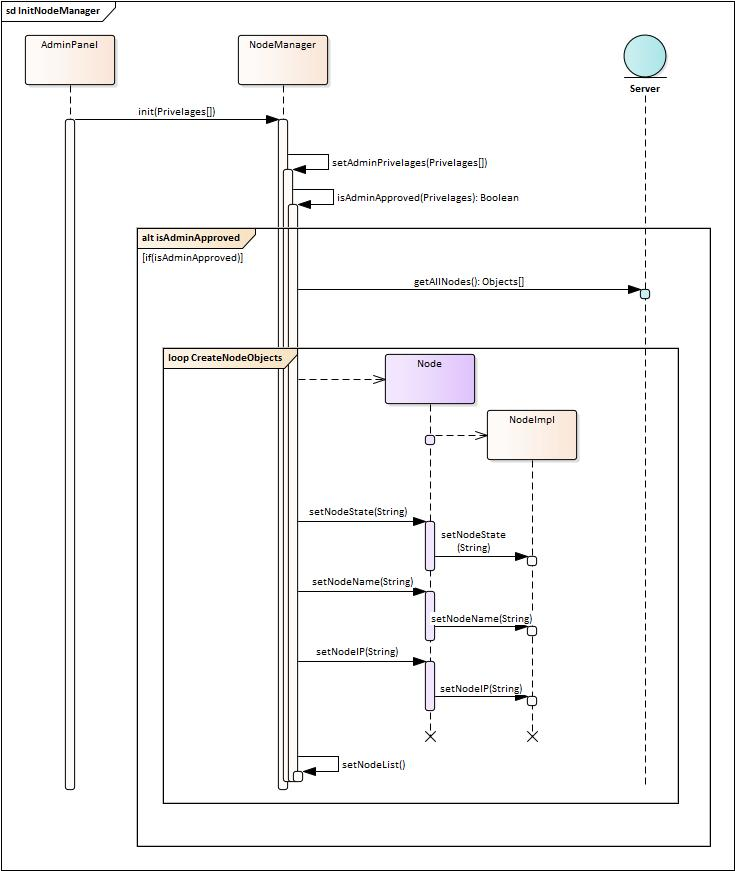
\includegraphics[width=12cm,height=20cm,keepaspectratio]{admin_ui/images/sequence_diagrams/InitNodeManager.jpg}
	\begin{center}
	    \small{Figure 27: Initialize Node Sequence Diagram}
    \end{center}
    
    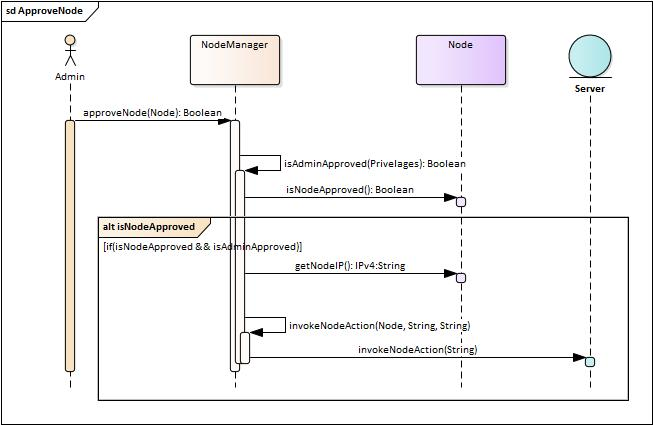
\includegraphics[width=15cm,height=15cm,keepaspectratio]{admin_ui/images/sequence_diagrams/ApproveNode.jpg}
	\begin{center}
	    \small{Figure 28: Approve Node Sequence Diagram}
    \end{center}
    
    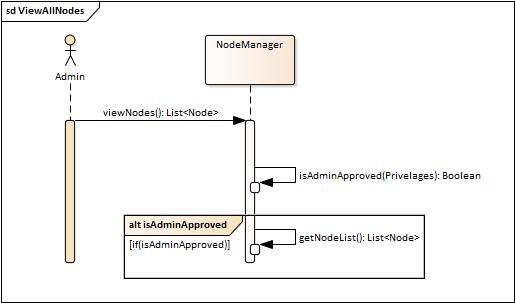
\includegraphics[width=12cm,height=15cm,keepaspectratio]{admin_ui/images/sequence_diagrams/ViewAllNodes.jpg}
	\begin{center}
	    \small{Figure 29: View All Nodes Sequence Diagram}
    \end{center}
    
    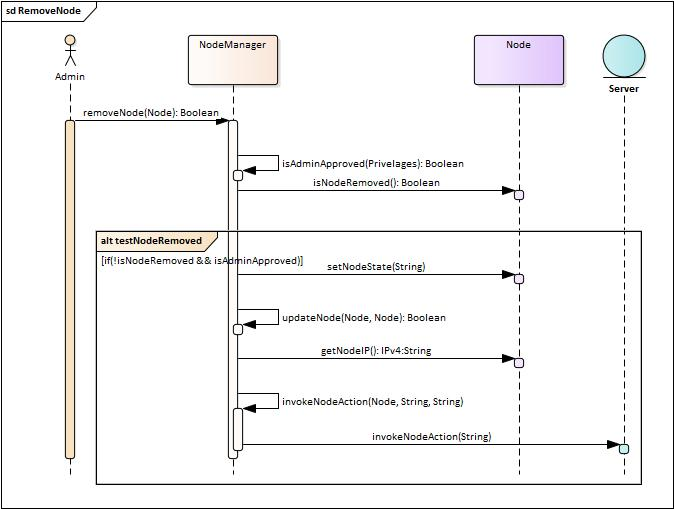
\includegraphics[width=13cm,height=15cm,keepaspectratio]{admin_ui/images/sequence_diagrams/RemoveNode.jpg}
		\begin{center}
	    \small{Figure 30: Remove Node Sequence Diagram}
    \end{center}
    
     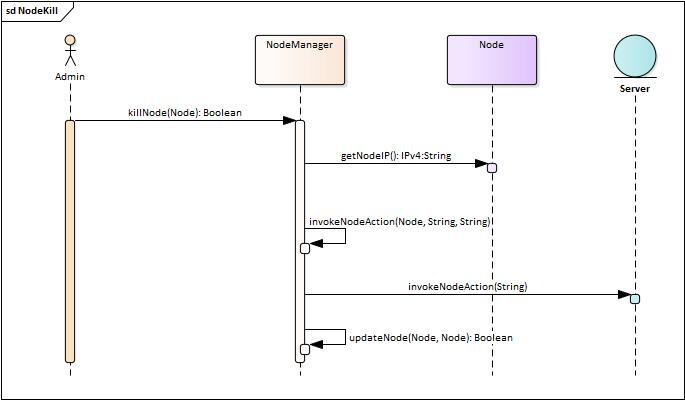
\includegraphics[width=13cm,height=15cm,keepaspectratio]{admin_ui/images/sequence_diagrams/NodeKill.jpg}
		\begin{center}
	    \small{Figure 31: Kill Node Sequence Diagram}
    \end{center}
    
    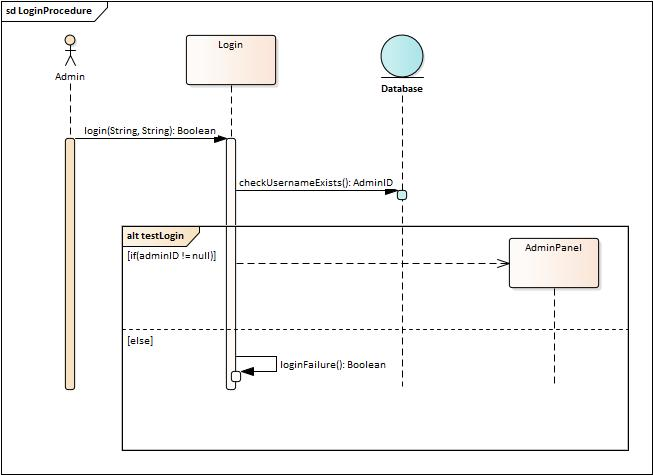
\includegraphics[width=12cm,height=15cm,keepaspectratio]{admin_ui/images/sequence_diagrams/LoginProcedure.jpg}
		\begin{center}
	    \small{Figure 32: Login Sequence Diagram}
    \end{center}
    
    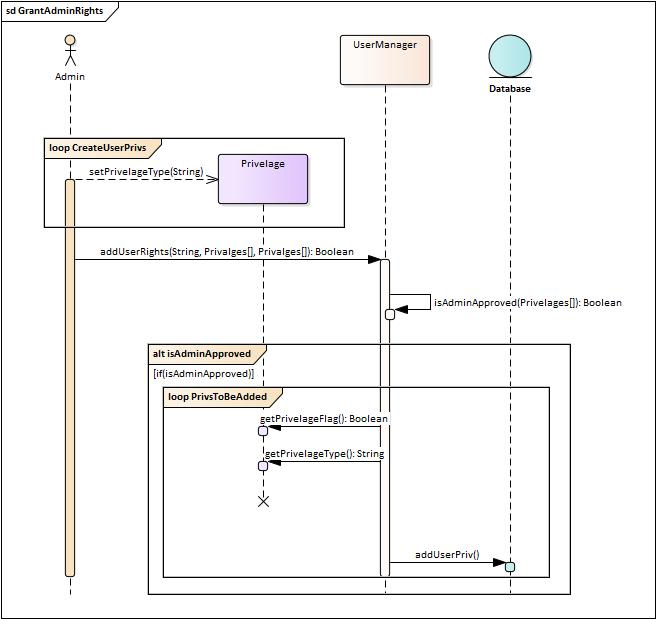
\includegraphics[width=12cm,height=15cm,keepaspectratio]{admin_ui/images/sequence_diagrams/GrantAdminRights.jpg}
		\begin{center}
	    \small{Figure 33: Grant Admin Rights Sequence Diagram}
    \end{center}
    
    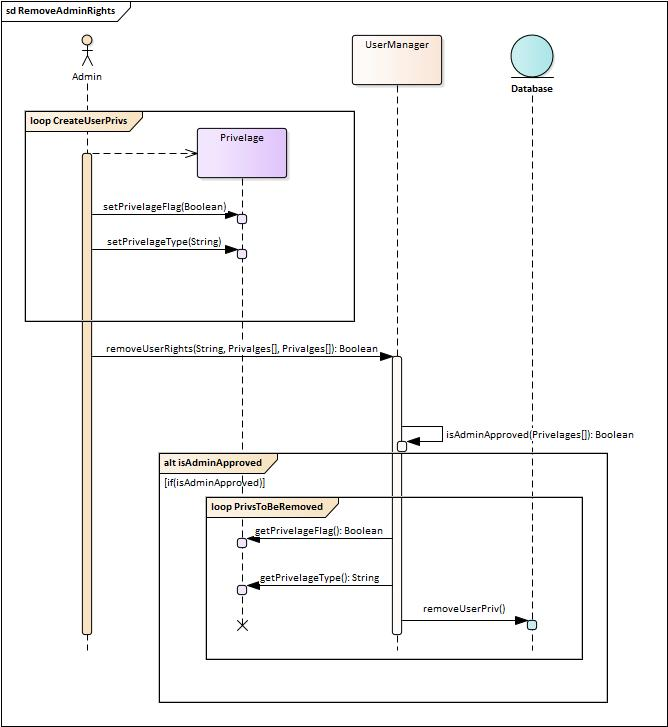
\includegraphics[width=12cm,height=15cm,keepaspectratio]{admin_ui/images/sequence_diagrams/RemoveAdminRights.jpg}
		\begin{center}
	    \small{Figure 34: Remove Admin Rights Sequence Diagram}
    \end{center}
    
    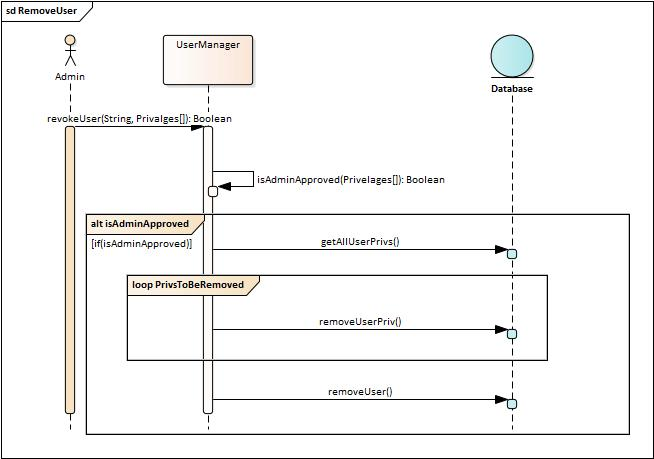
\includegraphics[width=12cm,height=15cm,keepaspectratio]{admin_ui/images/sequence_diagrams/RemoveUser.jpg}
		\begin{center}
	    \small{Figure 35: Remove User Sequence Diagram}
    \end{center}




\subsection{State diagram}
    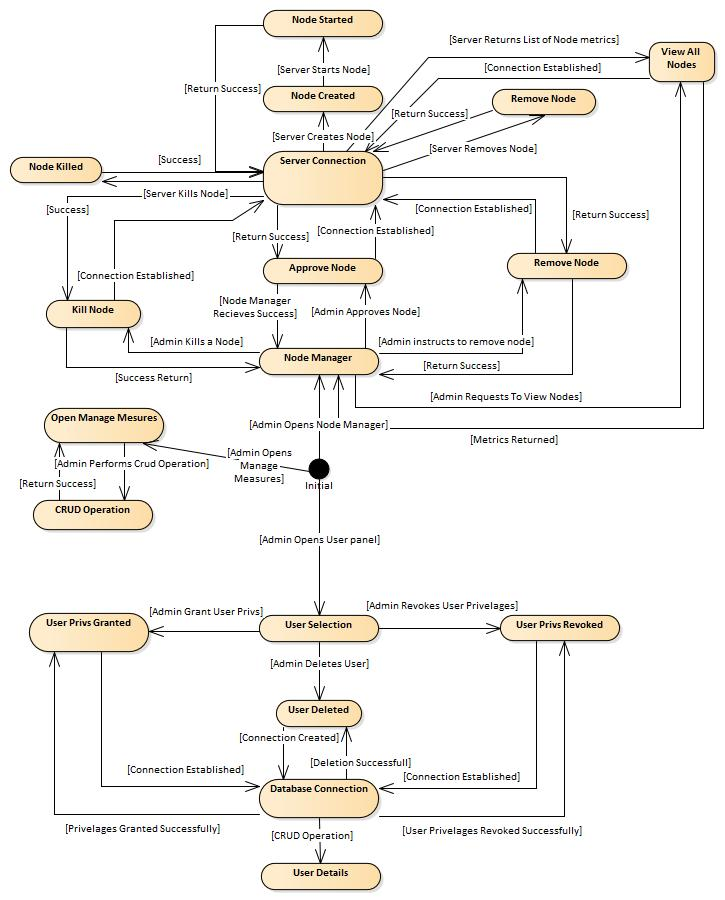
\includegraphics[width=12cm,height=15cm,keepaspectratio]{admin_ui/images/State_Diagram.jpg}
		\begin{center}
	    \small{Figure 36: State Diagram for Admin UI}
    \end{center}




\subsection{Use Case diagram}
    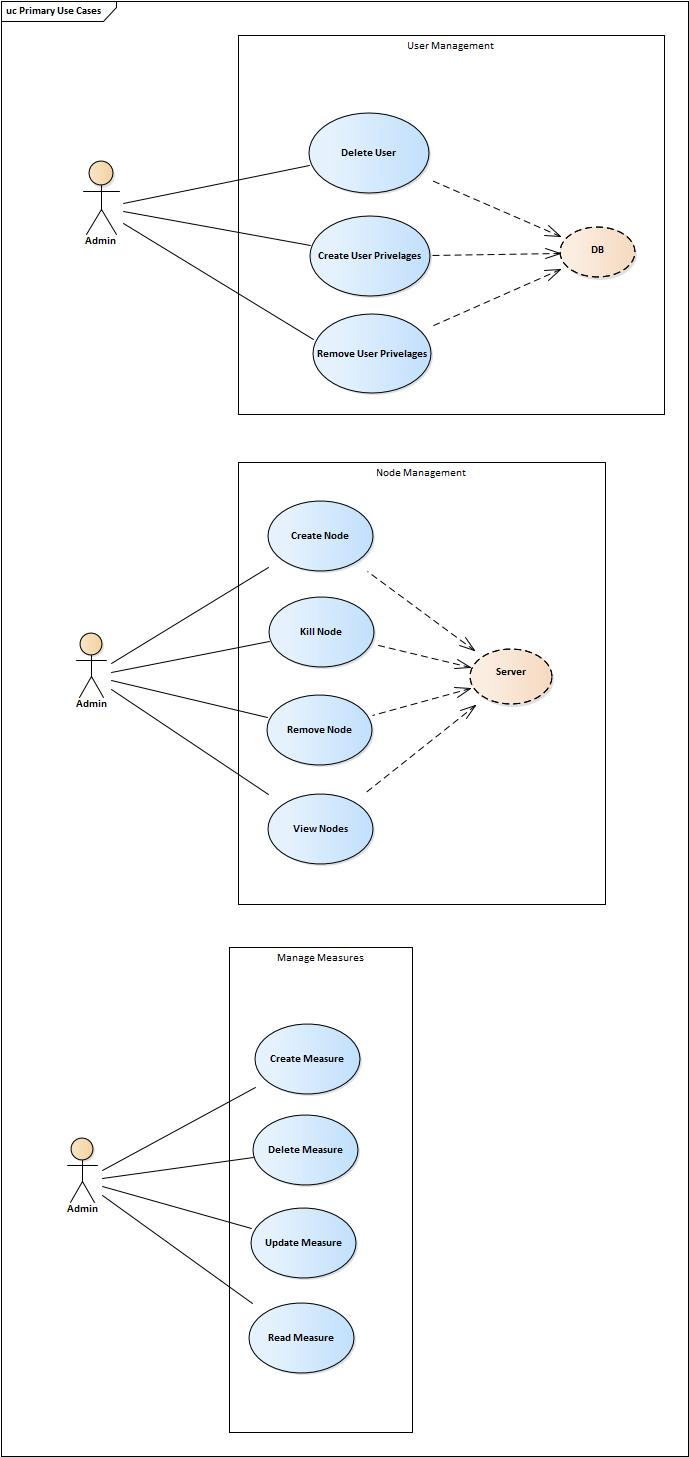
\includegraphics[width=12cm,height=15cm,keepaspectratio]{admin_ui/images/Primary_Use_Cases.png}
    \begin{center}
    	\small{Figure 37: Use case diagram for Admin UI}
    \end{center}